\documentclass[14pt]{extbook}
\usepackage{multicol, enumerate, enumitem, hyperref, color, soul, setspace, parskip, fancyhdr} %General Packages
\usepackage{amssymb, amsthm, amsmath, latexsym, units, mathtools} %Math Packages
\everymath{\displaystyle} %All math in Display Style
% Packages with additional options
\usepackage[headsep=0.5cm,headheight=12pt, left=1 in,right= 1 in,top= 1 in,bottom= 1 in]{geometry}
\usepackage[usenames,dvipsnames]{xcolor}
\usepackage{dashrule}  % Package to use the command below to create lines between items
\newcommand{\litem}[1]{\item#1\hspace*{-1cm}\rule{\textwidth}{0.4pt}}
\pagestyle{fancy}
\lhead{Progress Quiz 6}
\chead{}
\rhead{Version A}
\lfoot{1430-1829}
\cfoot{}
\rfoot{test}
\begin{document}

\begin{enumerate}
\litem{
Determine the domain of the function below.\[ f(x) = \frac{5}{18x^{2} -39 x + 20} \]\begin{enumerate}[label=\Alph*.]
\item \( \text{All Real numbers except } x = a, \text{ where } a \in [11.91, 12.04] \)
\item \( \text{All Real numbers except } x = a, \text{ where } a \in [0.74, 0.97] \)
\item \( \text{All Real numbers.} \)
\item \( \text{All Real numbers except } x = a \text{ and } x = b, \text{ where } a \in [0.74, 0.97] \text{ and } b \in [1.28, 1.61] \)
\item \( \text{All Real numbers except } x = a \text{ and } x = b, \text{ where } a \in [11.91, 12.04] \text{ and } b \in [29.82, 30.39] \)

\end{enumerate} }
\litem{
Solve the rational equation below. Then, choose the interval(s) that the solution(s) belongs to.\[ \frac{-80}{-40x -60} + 1 = \frac{-80}{-40x -60} \]\begin{enumerate}[label=\Alph*.]
\item \( \text{All solutions lead to invalid or complex values in the equation.} \)
\item \( x \in [-1.5,-0.5] \)
\item \( x_1 \in [-1.5, 0.5] \text{ and } x_2 \in [-2.5,0.5] \)
\item \( x_1 \in [-1.5, 0.5] \text{ and } x_2 \in [0.5,2.5] \)
\item \( x \in [0.5,3.5] \)

\end{enumerate} }
\litem{
Solve the rational equation below. Then, choose the interval(s) that the solution(s) belongs to.\[ \frac{2x + 0}{6x + 3} + \frac{-4x^{2} +0 x + 0}{-18x^{2} -33 x -12} = \frac{-2}{-3x -4} \]\begin{enumerate}[label=\Alph*.]
\item \( x_1 \in [-0.99, 0.35] \text{ and } x_2 \in [0.5,1.1] \)
\item \( x_1 \in [-0.99, 0.35] \text{ and } x_2 \in [-2,0.8] \)
\item \( x \in [-0.53,1.82] \)
\item \( \text{All solutions lead to invalid or complex values in the equation.} \)
\item \( x \in [-1.43,-0.7] \)

\end{enumerate} }
\litem{
Determine the domain of the function below.\[ f(x) = \frac{6}{15x^{2} -3 x -12} \]\begin{enumerate}[label=\Alph*.]
\item \( \text{All Real numbers.} \)
\item \( \text{All Real numbers except } x = a \text{ and } x = b, \text{ where } a \in [-2.1, 0.2] \text{ and } b \in [0.2, 2.2] \)
\item \( \text{All Real numbers except } x = a, \text{ where } a \in [-21.1, -19.6] \)
\item \( \text{All Real numbers except } x = a \text{ and } x = b, \text{ where } a \in [-21.1, -19.6] \text{ and } b \in [8.7, 9.5] \)
\item \( \text{All Real numbers except } x = a, \text{ where } a \in [-2.1, 0.2] \)

\end{enumerate} }
\litem{
Choose the equation of the function graphed below.
\begin{center}
    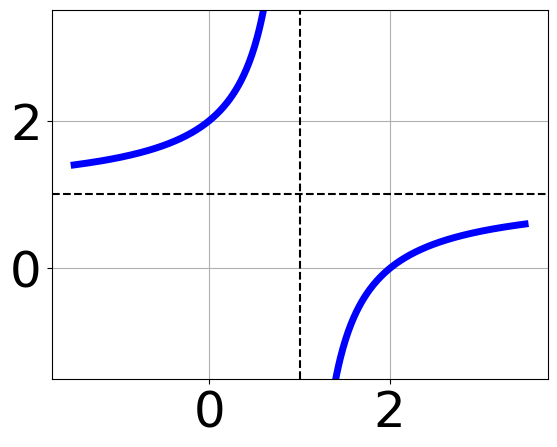
\includegraphics[width=0.5\textwidth]{../Figures/rationalGraphToEquationCopyA.png}
\end{center}
\begin{enumerate}[label=\Alph*.]
\item \( f(x) = \frac{1}{x + 1} + 7 \)
\item \( f(x) = \frac{1}{(x + 1)^2} + 7 \)
\item \( f(x) = \frac{-1}{x - 1} + 7 \)
\item \( f(x) = \frac{-1}{(x - 1)^2} + 7 \)
\item \( \text{None of the above} \)

\end{enumerate} }
\litem{
Choose the graph of the equation below.\[ f(x) = \frac{-1}{x - 2} - 3 \]\begin{enumerate}[label=\Alph*.]
\begin{multicols}{2}\item 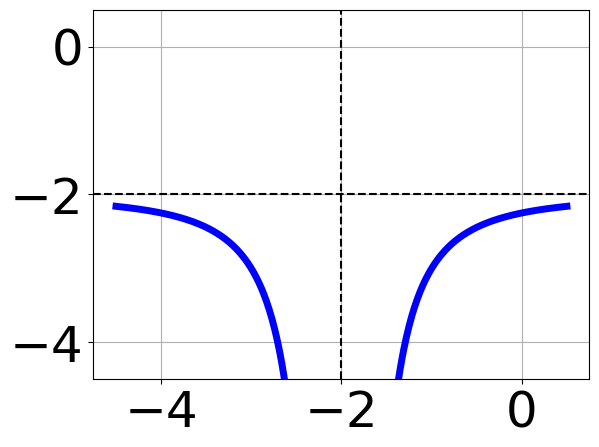
\includegraphics[width = 0.3\textwidth]{../Figures/rationalEquationToGraphAA.png}\item 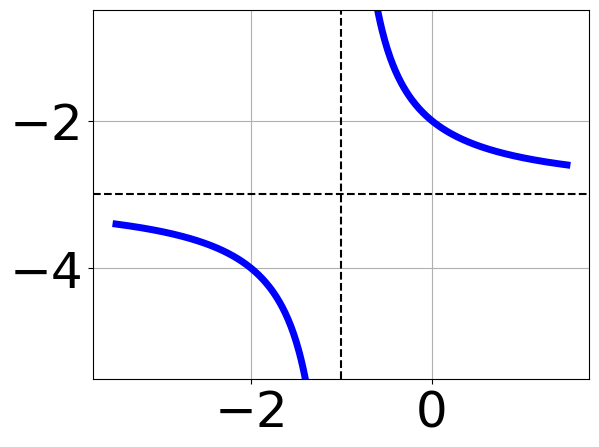
\includegraphics[width = 0.3\textwidth]{../Figures/rationalEquationToGraphBA.png}\item 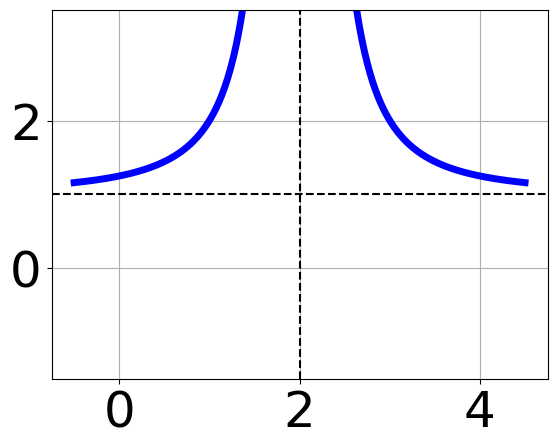
\includegraphics[width = 0.3\textwidth]{../Figures/rationalEquationToGraphCA.png}\item 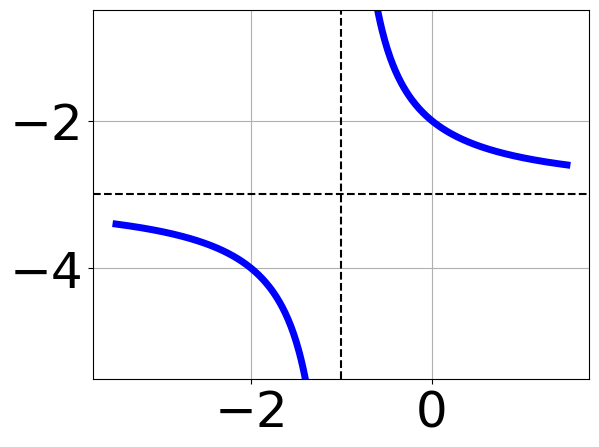
\includegraphics[width = 0.3\textwidth]{../Figures/rationalEquationToGraphDA.png}\end{multicols}\item None of the above.
\end{enumerate} }
\litem{
Solve the rational equation below. Then, choose the interval(s) that the solution(s) belongs to.\[ \frac{-117}{117x + 78} + 1 = \frac{-117}{117x + 78} \]\begin{enumerate}[label=\Alph*.]
\item \( x_1 \in [-1.1, 0.2] \text{ and } x_2 \in [0.3,1] \)
\item \( x_1 \in [-1.1, 0.2] \text{ and } x_2 \in [-2.3,-0.3] \)
\item \( x \in [-0.67,1.33] \)
\item \( \text{All solutions lead to invalid or complex values in the equation.} \)
\item \( x \in [-0.6,1.5] \)

\end{enumerate} }
\litem{
Choose the graph of the equation below.\[ f(x) = \frac{1}{(x + 2)^2} + 3 \]\begin{enumerate}[label=\Alph*.]
\begin{multicols}{2}\item 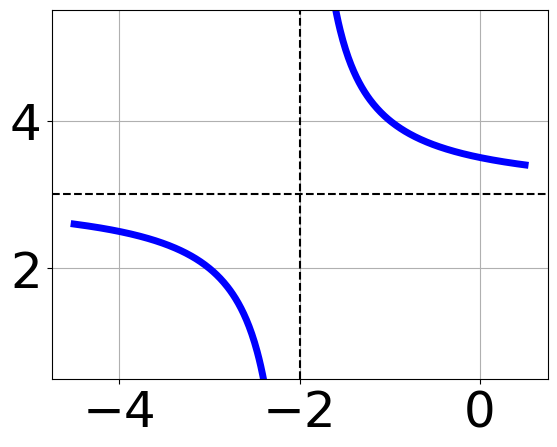
\includegraphics[width = 0.3\textwidth]{../Figures/rationalEquationToGraphCopyAA.png}\item 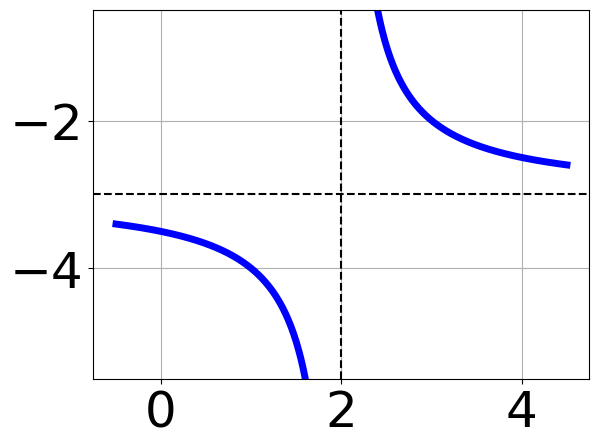
\includegraphics[width = 0.3\textwidth]{../Figures/rationalEquationToGraphCopyBA.png}\item 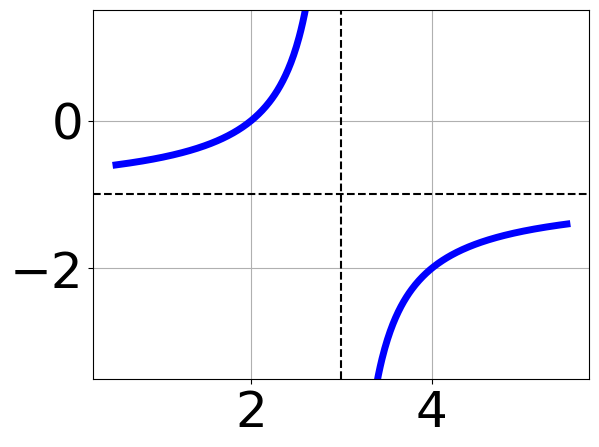
\includegraphics[width = 0.3\textwidth]{../Figures/rationalEquationToGraphCopyCA.png}\item 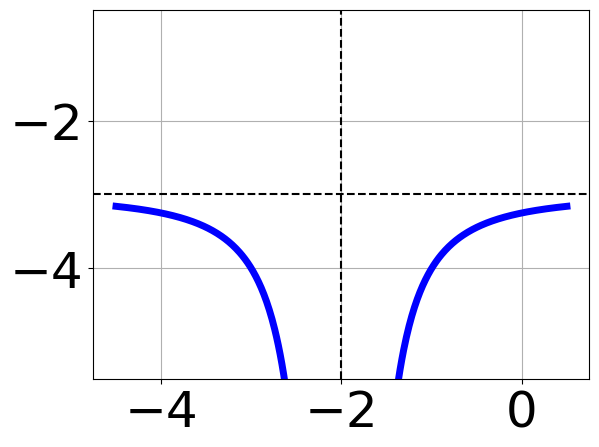
\includegraphics[width = 0.3\textwidth]{../Figures/rationalEquationToGraphCopyDA.png}\end{multicols}\item None of the above.
\end{enumerate} }
\litem{
Choose the equation of the function graphed below.
\begin{center}
    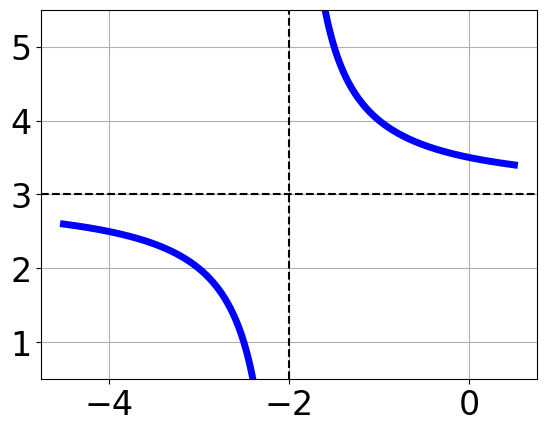
\includegraphics[width=0.5\textwidth]{../Figures/rationalGraphToEquationA.png}
\end{center}
\begin{enumerate}[label=\Alph*.]
\item \( f(x) = \frac{1}{x + 1} - 2 \)
\item \( f(x) = \frac{1}{(x + 1)^2} - 2 \)
\item \( f(x) = \frac{-1}{x - 1} - 2 \)
\item \( f(x) = \frac{-1}{(x - 1)^2} - 2 \)
\item \( \text{None of the above} \)

\end{enumerate} }
\litem{
Solve the rational equation below. Then, choose the interval(s) that the solution(s) belongs to.\[ \frac{6x + 0}{-5x -5} + \frac{-2x^{2} +0 x + 0}{-10x^{2} +25 x + 35} = \frac{2}{2x -7} \]\begin{enumerate}[label=\Alph*.]
\item \( \text{All solutions lead to invalid or complex values in the equation.} \)
\item \( x_1 \in [0.14, 0.96] \text{ and } x_2 \in [-2.4,0.9] \)
\item \( x \in [2.86,3.56] \)
\item \( x \in [2.1,3.45] \)
\item \( x_1 \in [0.14, 0.96] \text{ and } x_2 \in [1.5,3.2] \)

\end{enumerate} }
\end{enumerate}

\end{document}